% !TEX root = paper.tex

\documentclass[11pt,a4paper]{article}

% ====== PACKAGES ======
\usepackage[utf8]{inputenc}    % For UTF-8 encoding
\usepackage[T1]{fontenc}
\usepackage{graphicx}          % For including images
\usepackage{amsmath, amssymb}  % For math symbols
\usepackage{siunitx}           % For units
\usepackage{geometry}          % Page layout
\usepackage{hyperref}          % Clickable links
\usepackage{natbib}            % For references
\usepackage{setspace}          % Line spacing
\usepackage{booktabs}           % For professional tables
\usepackage{tabularx}            % For adjustable column widths

% ====== PAGE SETTINGS ======
\geometry{margin=1in}
\setstretch{1.2}

% ====== TITLE INFO ======
\title{Drawing agent experiments results}
\author{Guglielmo Montone}
\date{\today}

% ====== DOCUMENT START ======
\begin{document}

\maketitle

\section{Scope}
In the context of a drawing agent, we aim to show that an architecture trained to encode both the visual input (the drawing) and the action used to produce it can generalize better in a visual classification task than an architecture trained solely on visual input.
To test this hypothesis, we trained a V-JEPA architecture on videos of a drawing agent. The model received the first $T$ frames of each video and was asked to predict frame $T+1$. In one experiment (the action-access condition), the architecture was trained on the drawing videos with an additional small overlay showing the next action the agent would take. In the second experiment (the no-action-access condition), the architecture was trained only on the drawing frames, without access to the action information.
After training in both conditions, we used the encoders from each architecture in a downstream classification task. The classifier was asked to recognize drawing shapes, where each class consisted of a base shape along with random translations of that shape.
We expected that the V-JEPA architecture trained with access to the next-action encodings (action-access) would be more robust to translations. The results suggest that this is indeed the case, although the classification task may have been too easy overall, making the effect less pronounced.

\section{Datasets}
We defined three datasets one to train the V-JEPA architecture in the action-access condition, on the train it in the no-action-access condition and 
one to evaluate the performance of the trained models on a downstream classification task.
The first datasetconsists of videos of a drawing agent in which both the drawing and a representation of the agent’s action are visible. 
In the image below (Figure~\ref{fig:video_frames}) A and B we extract 4 frames from 2 of the videos in the dataset. 
The line at the center of the frame shows the actual drawing, while the four lines at the top encode the action the agent is taking.
To represent the action at frame $T$, we compute the difference between the last drawn point and the point that will be drawn at frames $T+2$, $T+4$, $T+6$, and $T+8$. These differences correspond to the four action lines shown from left to right.

\begin{figure}[h!]
    \centering
    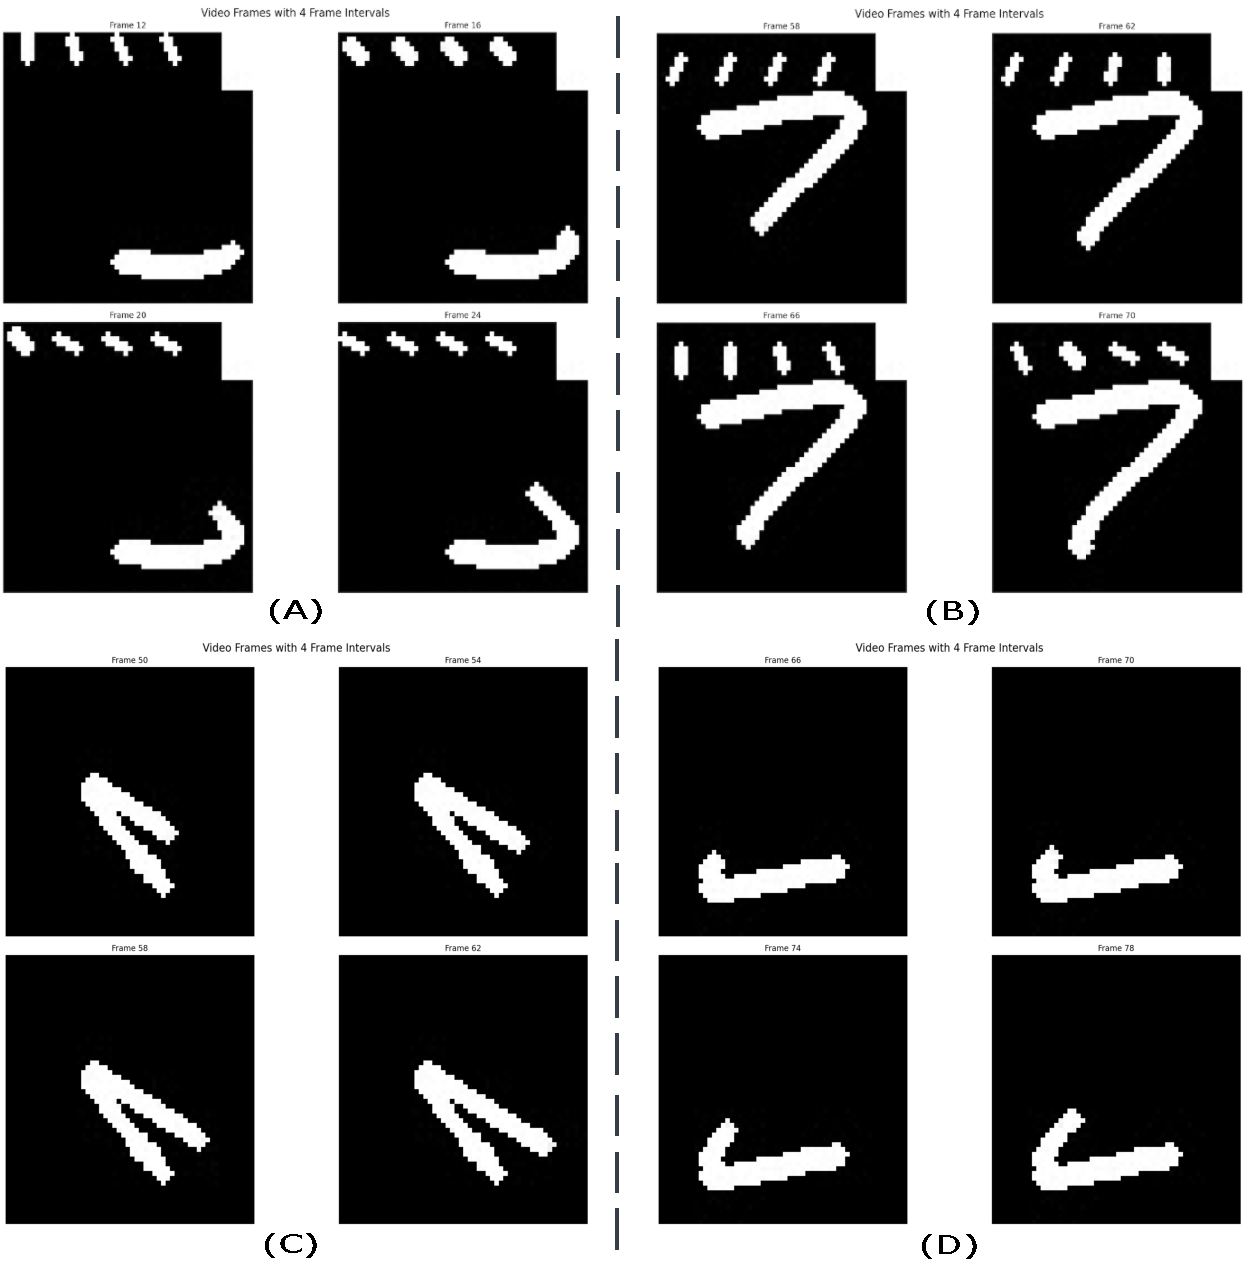
\includegraphics[width=0.8\textwidth]{experiment_2.pdf}
    \caption{Four consecutive frames from a drawing agent video.}
    \label{fig:video_frames}
\end{figure}

The second dataset (no-action-access) is similar to the first but does not include any action representation at the top. An example is 
shown in Figure~\ref{fig:video_frames} C and D.

The drawing in the videos for both the action-access and no-action-access datasets are generated by randomly selecting 
4 to 6 points on the drawing surface and connecting them using a smooth interpolation. 
Each video lasts 3 seconds and is recorded at 30 fps, resulting in a drawing trajectory composed of 90 points.
Each of the two datasets (action-access and no-action-access) is composed of 192K videos.

A third dataset is used to evaluate the quality of the learned representations. 
In particular, we were interested in testing whether the encoder trained on videos that included the action representation 
would generalize better. Specifically, we expected that this encoder would be more robust to translations—i.e., better at 
recognizing the same shape when it appears in different locations on the drawing surface. Our hypothesis is that the action
representation remains consistent across translations, and therefore should encourage the encoder to learn features that are invariant to the position of the shape.

\begin{figure}[h!]
    \centering
    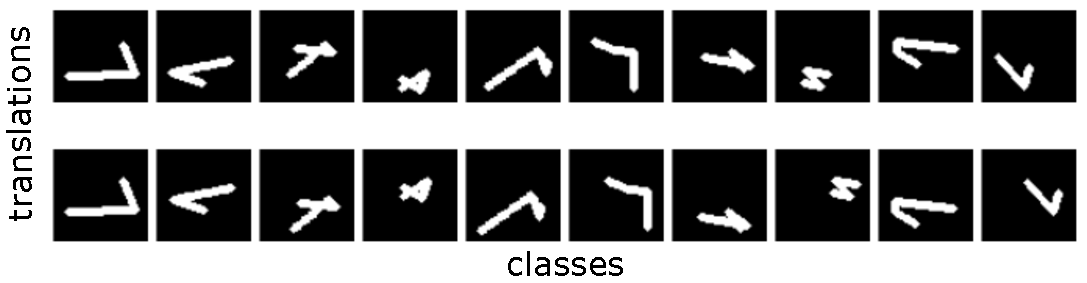
\includegraphics[width=0.8\textwidth]{experiment_3.pdf}
    \caption{Examples of the drawing present int the different classes of the dataset.}
    \label{fig:classes_examples}
\end{figure}

Three variations of the third dataset were created as follows:
\begin{itemize}
    \item 10-class dataset (80 samples per class)
    \item 20-class dataset (40 samples per class)
    \item 40-class dataset (20 samples per class)
\end{itemize}
These three datasets are designed to make the classification task increasingly challenging by simultaneously increasing the number of classes and reducing the number of examples available for each class.


\section{Results}
Here are the results of the classification task on the three different datasets.

\begin{table}[h!]
    \centering
    \begin{tabularx}{\textwidth}{lXXX}
        \toprule
        & \textbf{10-classes-dataset} & \textbf{20-classes-dataset} & \textbf{40-classes-dataset} \\
        \midrule
        no-action-access & 100\% & 97.5\% (155) & 86.6\% (278) \\
        action-access & 100\% & 96.8\% (156) & 90.2\% (288) \\
        \bottomrule
    \end{tabularx}
    \caption{Classification results across different dataset sizes. The accuracy and the number of correct predictions are reported for the best model on each dataset.}
    \label{tab:results}
\end{table}


% ====== REFERENCES ======
\bibliographystyle{plainnat}
\bibliography{references}

\end{document}